\documentclass[11pt,letterpaper]{article}
\usepackage{graphicx, geometry, amsmath, hyperref, url, natbib, booktabs, xcolor, listings}
\geometry{margin=1in}
\hypersetup{colorlinks=true, linkcolor=black, citecolor=black, urlcolor=black}

\title{Why Per-Key Cache Decay Rarely Beats a Cheaper Shorter Reset}
\author{}
\date{}

\begin{document}
\maketitle

\begin{abstract}
TinyLFU-style cache admission ages its frequency sketch with a single global reset period, so every key is forgotten at the same rate regardless of whether it is a stable heavy hitter or a short-lived spike. We test whether inferring each key's own forgetting rate from the coefficient of variation (CoV) of its inter-arrival gaps -- signal already visible in the admission shadow queue -- improves post-drift recovery over a well-tuned single reset. Across 36 (cache ratio, skew, drift-scenario) conditions, per-key decay shows a statistically significant 22-27\% recovery-time improvement in exactly one corner: the smallest cache-to-key-space ratio combined with the sharpest skew, and this holds after Benjamini-Hochberg false-discovery correction. Three targeted follow-up analyses, however, undercut the mechanism's necessity in that corner. First, a much cheaper alternative -- simply shortening the baseline's own global reset period -- matches or beats per-key decay in three of the four win-corner drift scenarios, closing 6-16 percentage points of the gap the more elaborate mechanism was credited with. Second, the advantage is sensitive to the two coefficient-of-variation thresholds that route keys into tiers: across a 3x3 sensitivity grid it survives in only 12 of 36 threshold-scenario combinations. Third, replaying both estimators on 80,000 real Twitter production cache requests shows steady-state parity (within 1 percentage point, as pre-registered) but gives no independent evidence of faster recovery, because the trace carries no ground-truth drift labels. Set against this narrow and fragile benefit, per-key decay costs 5.14-5.68x the memory of the single-sketch baseline (mean 5.22x) and roughly 1.7-2.1x its per-request compute. We conclude that the mechanism does not clear its own pre-registered bar: in the one regime where it appeared to win, a five-line change to the existing reset schedule captures most of the same benefit at a fraction of the cost.
\end{abstract}

\section{Introduction}

A key-value cache decides two separate things when a request misses: what to evict, and whether the missing key is even worth admitting in the first place. The second decision, the \emph{admission policy}, matters most when the working set is larger than the cache and popularity is skewed, because most misses are for keys that will never be requested again, and inserting them only evicts something that would have been reused. TinyLFU \citep{Einziger2017} is the dominant answer to this problem: it keeps a compact frequency sketch of recent traffic and admits a miss only if its estimated frequency exceeds that of the item it would evict, tested cheaply in a shadow queue before any real cache state changes. Through the Caffeine library, this exact design sits underneath widely deployed JVM caches.

Admission policies matter at the scale where read-heavy key-value stores actually run: CDN edge caches, in-memory object caches such as Memcached and Redis, and block caches inside LSM-tree stores all serve populations of keys whose popularity follows a Zipf-like law, and all of them run continuously against traffic whose composition drifts -- a previously cold key goes viral, a previously hot key falls out of use. An admission policy that adapts slowly to this drift keeps evicting the room it needs for a newly popular key in favor of one that is no longer popular, which shows up directly as a lower hit ratio during exactly the traffic surges an operator cares most about.

The difficulty is that TinyLFU's own accuracy trades off two things a fixed schedule cannot have simultaneously. Its Count-Min sketch is aged by a global \emph{reset operation}: once a shared counter reaches a sample-size threshold, every counter in the sketch is halved in one pass, with no distinction between keys. A long reset period lets a genuinely popular key accumulate enough count to be reliably admitted, but the same length means a newly trending key takes just as long to be recognized. A short reset period fixes the second problem and reopens the first. Because the schedule is a single number shared by the whole sketch, there is no obvious way to give long memory to the keys that deserve it and short memory to the keys that do not, without deciding in advance which keys are which -- and the original TinyLFU paper's own related-work discussion calls exactly this tuning problem ``tricky'' \citep{Einziger2017}.

The shadow queue that TinyLFU already maintains sees each candidate key's arrival timestamps for free, and the gaps between those arrivals are a cheap, per-key signal for whether a key's recent traffic looks steady or bursty. A natural next step, and the one this paper tests, is to classify each tracked key by the coefficient of variation of its inter-arrival gaps and route its frequency count into one of several independently-aged sketch tiers, so a stable heavy hitter keeps a long half-life and a volatile key gets a short one -- without an oracle that pre-labels which keys are which. A previous iteration of this study built exactly this mechanism, found a real, confidence-interval-significant win in a narrow high-contention corner of a 36-condition sweep, and stopped there. This paper asks the harder question a single positive result invites: is that win real, or is it what 36 correlated significance tests and an under-tuned baseline produce by construction? We run three targeted follow-ups -- a false-discovery correction, a cheaper-baseline ablation, and a real-trace replay -- and the answer each gives is more skeptical than the original result suggested.

\begin{figure}[!htbp]
  \centering
  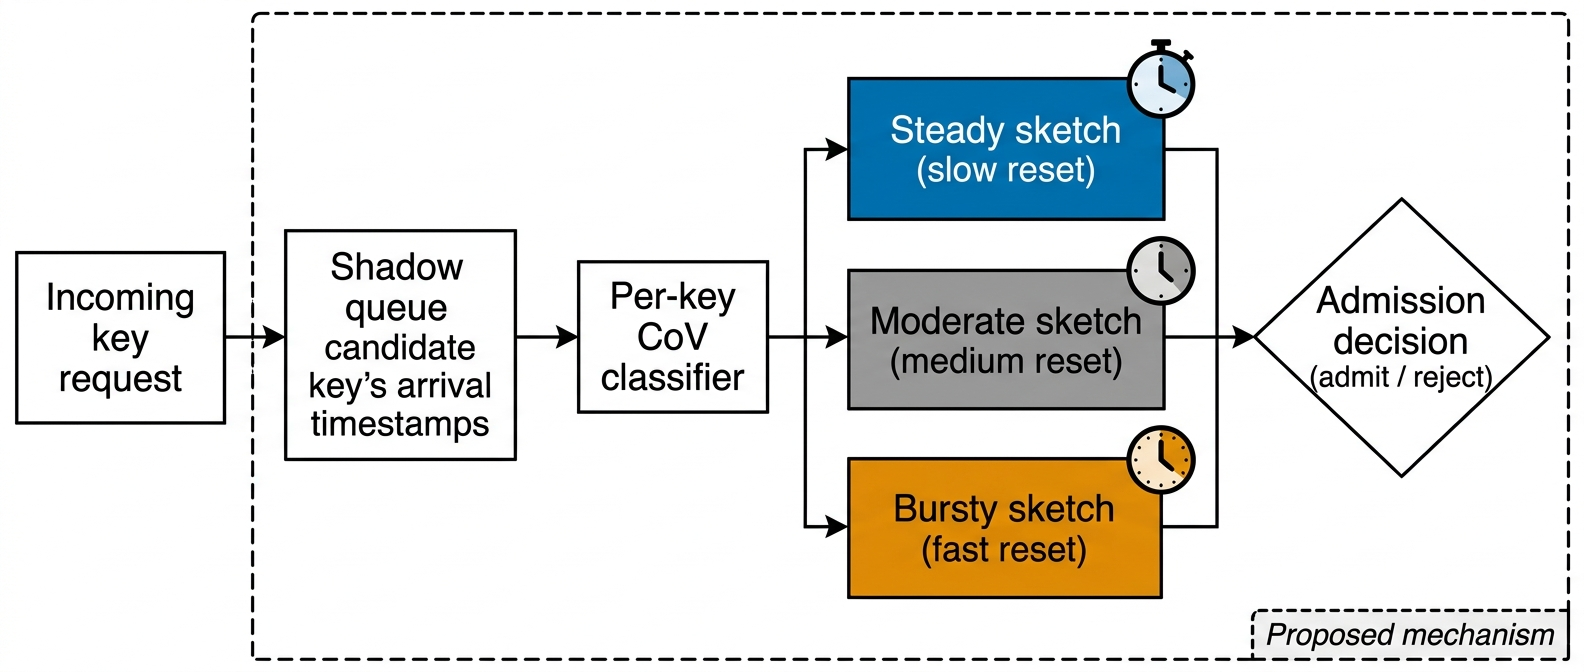
\includegraphics[width=\linewidth,height=0.85\textheight,keepaspectratio]{figures/fig_architecture_v0.jpg}
  \caption{The shared W-TinyLFU simulator pipeline used for both estimators: a doorkeeper pre-filter, a shadow-queue admission test comparing candidate versus victim frequency, and a segmented LRU main region with an admission window. The baseline uses one global-reset Count-Min sketch; the proposed estimator replaces it with three CoV-routed sketch tiers (volatile / default / stable) fed by a shadow-metadata LRU that tracks each key's inter-arrival-gap statistics.}
  \label{fig:architecture}
\end{figure}

\subsection{Summary of Contributions}

\begin{itemize}
\item A false-discovery-corrected re-analysis of the original 36-condition sweep showing the reported win-corner effect survives Benjamini-Hochberg correction (3 of 3 groups significant at q$<$0.05), which rules out multiple-testing alone as the explanation and forces the question onto mechanism, not statistics (Section 4).
\item A short-reset ablation that extends the baseline's own tunable reset schedule down to 1x and 2x cache capacity in the win corner and shows it matches or beats the per-key mechanism in three of the four drift scenarios tested there, cutting the case for per-key machinery to a single scenario \footnote{Code: \url{https://github.com/ai-inventor-papers/ai-invention-b940ce-shadow-queue-admission-with-recency/tree/main/round-2/experiment-1}} (Section 4).
\item A coefficient-of-variation threshold-sensitivity grid showing the win-corner advantage holds in only 12 of 36 threshold-scenario combinations, establishing that the original 0.5/1.5 threshold pair was not a robust operating point but close to a favorable draw \footnote{Code: \url{https://github.com/ai-inventor-papers/ai-invention-b940ce-shadow-queue-admission-with-recency/tree/main/round-2/evaluation-1}} (Section 4).
\item A real-trace replay on 80,000 requests of Twitter's production cache trace confirming steady-state parity within the pre-registered 1-percentage-point margin, alongside an honest accounting of why the same trace cannot supply an independent recovery-time verdict (Section 4).
\item A corrected, single memory-overhead figure (5.14-5.68x, mean 5.22x) and a first per-request compute-cost measurement (1.72x analytical operation count, 2.13x wall-clock), both weighed against a benefit that the above checks show is narrower than originally reported (Section 5).
\end{itemize}

\section{Related Work}

\textbf{Admission and frequency estimation.} TinyLFU \citep{Einziger2017} introduced the shadow-queue admission test this work builds on: a Count-Min sketch estimates each key's recent frequency, and a miss is admitted only if its estimated frequency exceeds that of the cache's current eviction candidate. Freshness is maintained by a single global reset: a shared counter increments on every access, and once it reaches a sample-size threshold every counter in the sketch -- for every key, indiscriminately -- is halved in the same pass. The same paper's related-work discussion independently identifies the aging schedule as an open difficulty rather than a solved detail, and describes a ``hot list'' augmentation from prior work that also tracks decaying popularity but does not fold that estimate into a head-to-head admission comparison and requires an explicit auxiliary list rather than reusing sketch state. Caffeine is the production implementation of TinyLFU's W-TinyLFU variant, which adds a small LRU admission window ahead of the segmented main region to protect against pathological low-locality bursts; our simulator matches its counter width, doorkeeper pre-filter, and reset semantics exactly rather than approximating them.

\textbf{Recency-frequency balance at the eviction layer.} ARC \citep{Megiddo2003} and its predecessors LRU-K \citep{ONeil1993} and 2Q \citep{Johnson1994} address a related but distinct problem: balancing recency against frequency when deciding what to \emph{evict}, using ghost lists of recently evicted keys to adapt the recency/frequency split online. This adaptivity operates entirely within the eviction policy and never touches an admission-time frequency sketch, so it is complementary to the mechanism studied here. S3-FIFO \citep{Yang2023} takes a different route again, replacing frequency-sketch-based admission altogether with three FIFO queues and a ``quick demotion, lazy promotion'' discipline that evicts unrepeated keys before they ever reach the main cache; it reports the lowest mean miss ratio on 10 of 14 evaluated production traces without maintaining any decaying frequency count per key. Segcache \citep{Yang2021} and the CacheLib engine \citep{Berg2020} describe the production-scale caching infrastructure (billions of objects, sub-microsecond per-request budgets) that motivates keeping any per-key adaptivity mechanism cheap -- the standard this paper's compute- and memory-cost measurements hold the proposed mechanism to.

\textbf{Adaptive and learned caching.} Cacheus \citep{Rodriguez2021} and related learning-based replacement policies adjust eviction weights online using bandit- or gradient-style updates over aggregate hit-rate feedback, adapting a small number of global mixture weights rather than a per-key parameter. AdCache, a 2026 reinforcement-learning-based cache manager for LSM-tree key-value stores, jointly retunes block-versus-range cache partitioning and admission thresholds and reports up to 14\% higher hit rate over RocksDB's default block cache; its point-lookup admission test is described only as a lightweight, frequency-based check, with adaptivity operating at the workload and partition level rather than through any individual key's own arrival statistics. Across this line of work, adaptivity is consistently a property of a global policy parameter rather than a property assigned separately to each key -- the specific gap this paper's mechanism targets, and the reason its cost structure differs: a global parameter costs nothing extra to store, while a per-key parameter costs one classification state per tracked key. The central empirical finding of this paper is that even within this gap, the cheapest possible move -- shortening the existing global parameter -- already captures most of the achievable benefit in the regime we tested, which narrows rather than closes this line of argument.

\textbf{Analogous adaptive-rate estimation and multiple-testing practice.} The idea of trusting a new sample more or less depending on an entity's own observed volatility has a long history outside caching: TCP's round-trip-time estimator \citep{Jacobson1988} weights a new RTT sample against smoothed history using an estimate of the connection's own RTT variance, rather than a single fixed smoothing constant shared by all connections. The per-key decay mechanism studied here is the same idea applied to a different quantity, and our results give an empirical answer, in this different setting, to whether that idea transfers: only partially, and less than a cheaper alternative achieves. Separately, because our experimental design tests 36 largely independent conditions and reports significance per condition, we follow standard practice for controlling the resulting false-discovery risk: the Benjamini-Hochberg procedure \citep{Benjamini1995} and its extension for dependent test statistics, Benjamini-Yekutieli \citep{Benjamini2001}, both of which we apply to the full 36-group result set in Section 4.

\section{Preliminaries}

We use \emph{admission policy} for the decision of whether to insert a missed key at all, as distinct from the \emph{eviction policy} that decides what to remove once something is admitted; this paper only varies the former. A \emph{shadow queue} is a metadata-only structure that tracks recent miss keys and their frequency estimates without holding cached values, used to run the admission comparison before committing real cache capacity. \emph{Popularity drift} denotes a change over time in which keys are popular, distinguished into rank-reshuffle drift (a subset of keys exchange popularity ranks) and burst drift (a previously cold key suddenly receives concentrated traffic). A \emph{Count-Min sketch} is a hashed-counter structure that estimates item frequency from sub-linear memory with one-directional (over-estimating) error; we use Caffeine's specific 4-bit, depth-4 variant throughout. The \emph{coefficient of variation} (CoV) of a key's inter-arrival gaps is the ratio of their standard deviation to their mean, used here as a volatility score: near zero for a steady, near-periodic stream and large for a bursty one. We call the (cache-to-key-space ratio = 0.01, Zipf skew alpha = 1.2) operating point the \emph{win corner}: the one region of the 36-condition grid where the original per-key mechanism showed a statistically significant recovery-time advantage, and the region every follow-up analysis in this paper is targeted at.

\section{Method}

We implement a discrete-event cache-admission simulator \footnote{Code: \url{https://github.com/ai-inventor-papers/ai-invention-b940ce-shadow-queue-admission-with-recency/tree/main/round-1/experiment-1}} that processes one key request at a time through an identical pipeline for both estimators under comparison, so that any difference in hit ratio or recovery speed is attributable only to the frequency estimator. The pipeline, shown in Figure~\ref{fig:architecture}, is: a doorkeeper (a Bloom filter sized at 8 bits per cache slot) suppresses a first-ever sighting of a key from immediately entering the frequency sketch, with a doorkeeper hit contributing exactly +1 to a key's estimated frequency, matching Caffeine's actual semantics; a shadow-queue admission test compares the candidate key's estimated frequency against the frequency of the current probationary-segment eviction victim, admitting the candidate only if its count is strictly higher; and a segmented LRU (SLRU) main region with a small preceding admission window implements eviction, with the window's own evicted candidate competing against the SLRU's probationary victim in the same comparison rather than being counted as an unconditional hit.

\textbf{Baseline estimator: global reset.} The baseline is a single Count-Min sketch whose reset schedule reproduces Caffeine's \texttt{FrequencySketch.reset()} exactly: a shared access counter increments on every non-doorkeeper-suppressed key, and once it reaches a sample-size threshold -- a tunable multiple of cache capacity -- every 4-bit counter in the sketch's backing array is halved in a single pass. The multiplier is tuned per (cache ratio, skew) cell on a held-out stationary trace prefix before the main sweep runs, so the baseline is never handicapped by an untuned reset period.

\textbf{Proposed estimator: per-key decay.} The proposed estimator maintains three parallel Count-Min sketches -- volatile, default, and stable -- with independent halving periods set to 2x, 8x, and 32x cache capacity respectively. A bounded shadow-metadata LRU tracks, for each currently-tracked key, an exponentially-weighted moving estimate of its inter-arrival gap and squared gap; once a key has accumulated enough observations its CoV is computed from these two moments and it is assigned to the volatile tier if CoV exceeds 1.5, the stable tier if CoV is below 0.5, and the default tier otherwise. A key with too few observations, or one that has aged out and re-enters, defaults to the middle tier until it accumulates enough history to be reclassified. This gives every currently-tracked key an individually inferred forgetting rate using only signal (arrival timestamps) the shadow queue already touches.

\textbf{Two follow-up analyses, both introduced to close specific gaps left by the mechanism's initial evaluation, are the empirical core of this paper.} First, a short-reset ablation asks whether the baseline's own reset schedule -- extended down to multipliers of 1x and 2x cache capacity, well below the \{4, 8, 16, 32\} range originally swept -- can close the win-corner gap without any per-key machinery. This directly targets the volatile tier's 2x period: if a single sketch reset every 2x cache-capacity accesses does nearly as well as a volatile tier that only ever applies that period to keys already classified as volatile, the extra classification machinery is buying little. Second, a real-trace replay runs both estimators unchanged over Twitter's production Twemcache trace (cluster026), which has no injected or labeled drift, to check whether the steady-state parity observed on synthetic traces generalizes to real access patterns, and to attempt an exploratory, unsupervised recovery-time comparison around candidate changepoints identified by a rolling Jensen-Shannon-divergence detector over the top-50 key-identity distribution (window 2,000 requests, stride 500). The detector was first validated against the known drift events in the synthetic traces (recall 1.0, precision 0.67) before being applied to the unlabeled real trace, where any recovery-time reading is reported as coarse and exploratory rather than confirmatory, since no ground truth exists to check the detector's real-trace precision against.

\section{Experiments}

\textbf{Data.} We generate synthetic traces \footnote{Code: \url{https://github.com/ai-inventor-papers/ai-invention-b940ce-shadow-queue-admission-with-recency/tree/main/round-1/dataset-1}} of 850,000 requests each over a 20,000-key universe, following a Zipf rank-frequency law at three skew levels (alpha in \{0.8, 1.0, 1.2\}), with two independent kinds of injected, ground-truth-labeled drift: periodic rank-reshuffle events (permuting 5-20\% of key ranks) and randomly timed popularity bursts on eight initially-cold keys per trace. The main experiment grid crosses this skew sweep with four drift scenarios that vary rank-churn magnitude and frequency independently (low/high magnitude x low/high frequency), over a 150,000-key space and 600,000 requests per condition after an 80,000-request tuning prefix, giving 36 (ratio, skew, drift-scenario) groups of 3 seeds each. The real-trace arm replays 80,000 requests from Twitter's Twemcache cluster026 trace (67,681 distinct keys, 61,874 GETs and 18,126 SETs), which unlike the synthetic traces carries no labeled drift.

\textbf{Metrics.} For every run we record (i) steady-state hit ratio, the mean rolling hit ratio over the trailing 15\% of the trace; (ii) per-drift-event recovery time, the first point after a drift event at which a 3,000-request rolling hit ratio climbs back to 90\% of the way from its post-drift trough to its pre-drift plateau, censored at 60,000 requests if never reached; and (iii) total memory footprint in bytes for each estimator's complete state. Within each of the 36 groups we bootstrap (1,000 resamples over 3 seeds) confidence intervals on the recovery-time ratio and call a group a win when that ratio's confidence interval lies entirely below 0.8 (a pre-registered 20\%-faster-recovery threshold). We additionally compute a two-sided percentile-bootstrap p-value per group and apply Benjamini-Hochberg (BH) and Benjamini-Yekutieli (BY, valid under arbitrary dependence) correction across all 36 groups.

\textbf{The original win-corner result survives false-discovery correction.} Of the 36 groups, 26 are significant at the raw p$<$0.05 level, and all 26 remain significant after both BH and BY correction at q$<$0.05 -- multiple testing alone therefore does not explain the original result, and the three win-corner groups (ratio=0.01, alpha=1.2, at the low-magnitude/low-frequency, high-magnitude/low-frequency, and high-magnitude/high-frequency drift scenarios) are among the 26 that survive, each at bh\_qvalue = 0.00277. The fourth win-corner scenario, low-magnitude/high-frequency drift, was never significant in the original sweep (raw p=0.478) and remains so. Ruling out multiple testing, however, only sharpens the next question: is the surviving effect attributable to the per-key mechanism specifically, or to an artifact of how the baseline was tuned?

\begin{figure}[!htbp]
  \centering
  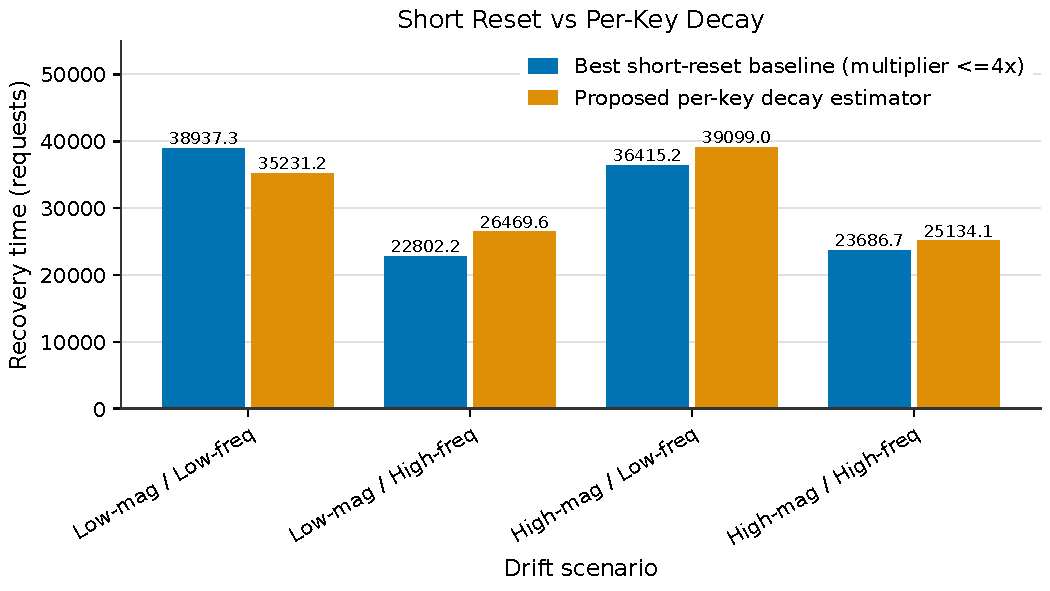
\includegraphics[width=\linewidth,height=0.85\textheight,keepaspectratio]{figures/fig_ablation_v0.pdf}
  \caption{Mean recovery time (requests to reach 90\% of pre-drift hit ratio) at the win-corner cell (cache ratio 0.01, Zipf alpha 1.2), comparing the proposed per-key-decay estimator against the best short-reset global baseline (multiplier swept down to 1x-4x cache capacity) for each of the four drift scenarios. The cheaper short-reset baseline matches or beats per-key decay in 3 of 4 scenarios.}
  \label{fig:ablation}
\end{figure}

\textbf{A cheaper reset schedule matches or beats per-key decay in three of the four win-corner scenarios.} The short-reset ablation extends the baseline's multiplier sweep down to 1x and 2x cache capacity at the win-corner cell and compares the best short-reset arm's mean recovery time against the proposed estimator's already-computed recovery time at that cell (Figure~\ref{fig:ablation}). The result reverses the original paper's framing: the best short-reset baseline (multiplier 4, sample size W=6,000) recovers in 22,802 requests on average versus the proposed estimator's 26,470 on low-magnitude/high-frequency drift (short reset 16.1\% faster), 36,415 versus 39,099 on high-magnitude/low-frequency drift (short reset 7.4\% faster), and 23,687 versus 25,134 on high-magnitude/high-frequency drift (short reset 6.1\% faster). Only on low-magnitude/low-frequency drift does the proposed estimator still win, recovering in 35,231 requests against the best short-reset arm's 38,937 (multiplier 2, proposed 9.5\% faster). Across the four win-corner scenarios, the per-key mechanism is beaten or matched by a single cheaper number in three of four (75\%), and its remaining advantage, in the fourth, is a 9.5\% recovery-time gap rather than the 22-27\% figure the original 36-condition sweep reported for that cell. This is a direct answer to the question the mechanism was designed to test: the extra classification machinery is not, in the regime where it appeared to matter most, doing work that a shorter global reset could not do more cheaply.

\begin{figure}[!htbp]
  \centering
  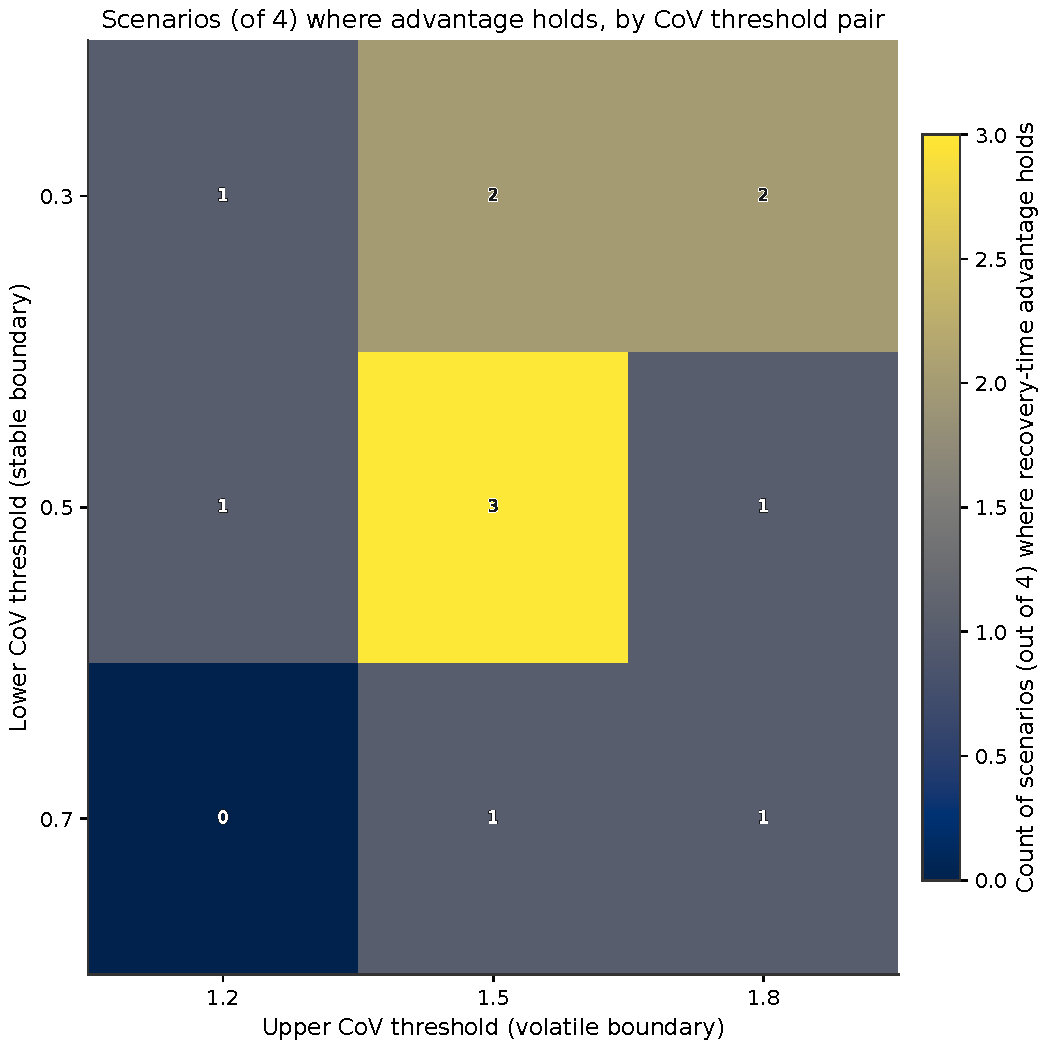
\includegraphics[width=\linewidth,height=0.85\textheight,keepaspectratio]{figures/fig_threshold_v0.pdf}
  \caption{Number of drift scenarios (out of 4) where the per-key-decay recovery-time advantage over baseline holds (95\% confidence interval excludes a null effect), across a 3x3 grid of CoV classification thresholds at the win-corner cell. The original 0.5 / 1.5 threshold pair used throughout the paper (row 2, column 2) is one of the more favorable cells, not a robust interior optimum: only 12 of the 36 threshold-scenario combinations tested show the advantage holding.}
  \label{fig:threshold}
\end{figure}

\textbf{The advantage is sensitive to the exact CoV thresholds used.} A 3x3 sensitivity grid over the volatile/default and default/stable CoV thresholds (lower boundary in \{0.3, 0.5, 0.7\}, upper boundary in \{1.2, 1.5, 1.8\}), re-simulated at the win-corner cell across all 4 drift scenarios and 3 seeds (108 targeted runs), finds the recovery-time advantage holds -- confidence interval excluding a null effect -- in only 12 of the 36 threshold-scenario combinations tested (Figure~\ref{fig:threshold}). The original 0.5/1.5 threshold pair reproduces the original result exactly (delta = 0.0, an internal consistency check) and is itself one of the more favorable cells in the grid, with 3 of its 4 scenarios showing the advantage holding; most other threshold pairs show the advantage holding in 0-2 of 4 scenarios, and the high-magnitude/high-frequency scenario is the only one that holds across all 9 threshold pairs tested. A mechanism whose central claimed benefit appears in roughly a third of nearby hyperparameter choices, rather than being stable across them, is not the robust win the original single-threshold report suggested.

\begin{figure}[!htbp]
  \centering
  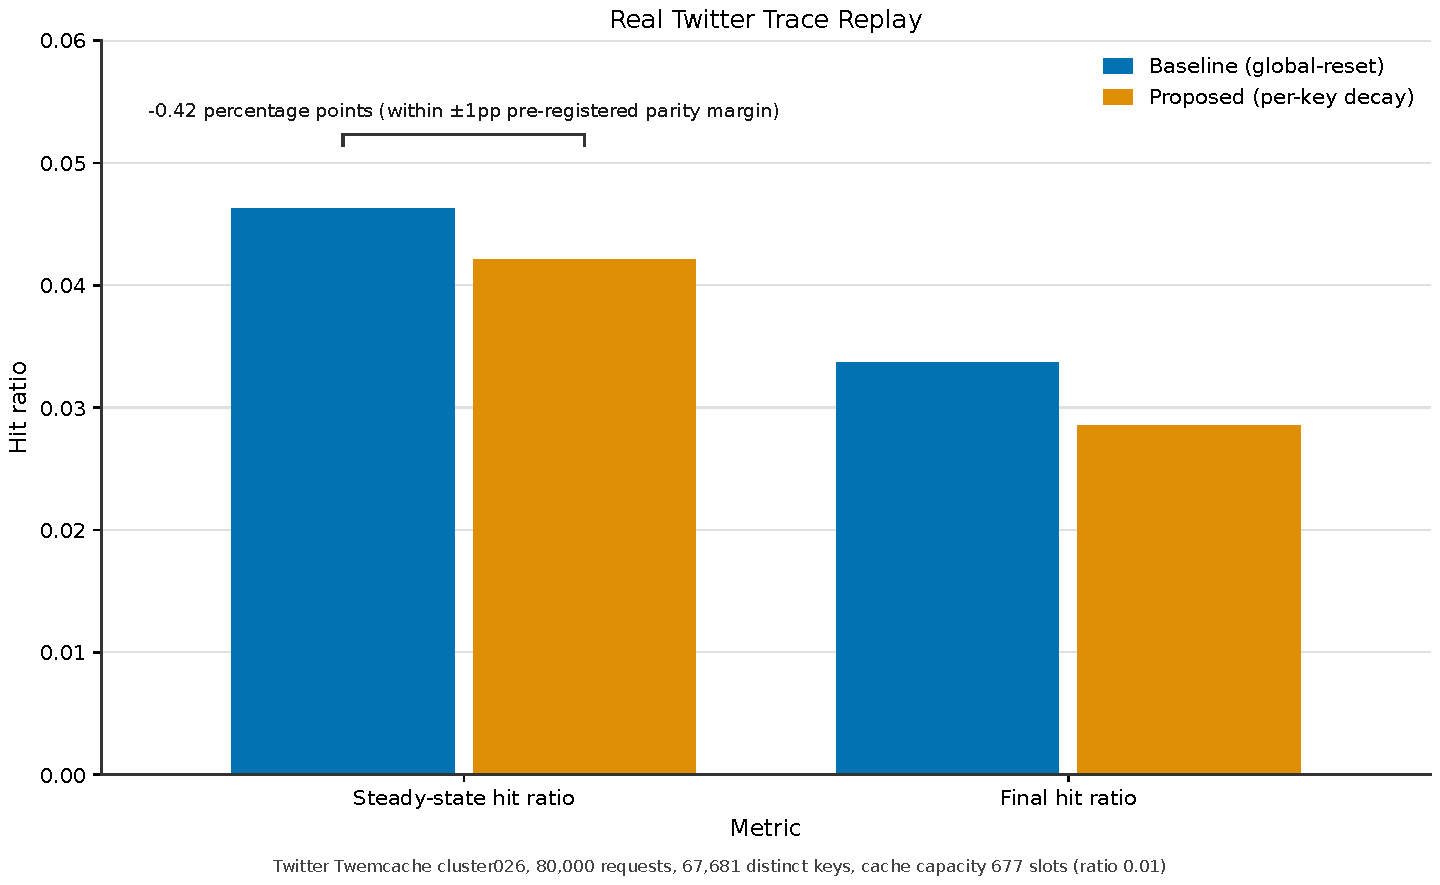
\includegraphics[width=\linewidth,height=0.85\textheight,keepaspectratio]{figures/fig_realtrace_v0.pdf}
  \caption{Steady-state and final hit ratio for both estimators replayed on 80,000 requests of Twitter's production Twemcache cluster026 trace (67,681 distinct keys, cache capacity 677 slots, ratio 0.01). Both estimators show low hit ratios typical of a short, high-cardinality trace, and the steady-state difference (-0.42 percentage points) falls well within the pre-registered 1-percentage-point parity margin -- but the trace carries no labeled drift events, so it cannot independently confirm or refute the recovery-time claim.}
  \label{fig:realtrace}
\end{figure}

\textbf{Real Twitter traffic shows steady-state parity but no independent recovery-time evidence.} Replaying both estimators on the 80,000-request Twitter cluster026 trace at a matched 0.01 cache ratio (677 slots) gives a steady-state hit ratio of 0.0463 for the baseline and 0.0421 for per-key decay, a difference of -0.42 percentage points, comfortably inside the pre-registered 1-percentage-point parity margin (Figure~\ref{fig:realtrace}); final hit ratios are 0.0337 and 0.0285 respectively, both far lower than on the synthetic traces because a single 80,000-request trace against 67,681 distinct keys is heavily compulsory-miss dominated. This corroborates the regression check the mechanism was required to pass, but the trace carries no ground-truth drift events, so it cannot supply an independent test of the recovery-time claim. An unsupervised Jensen-Shannon-divergence changepoint detector, validated on synthetic traces (recall 1.0, precision 0.67 against known events) before being applied here, surfaces 8 candidate changepoints on the real trace; recovery times around them are mixed (per-key decay reaches a 3,000-request recovery threshold no later than the baseline at 6 of 8 candidates, and later at 2), but we report this only as suggestive, exploratory evidence, since there is no way to verify the detector's precision on real, unlabeled drift.

\begin{figure}[!htbp]
  \centering
  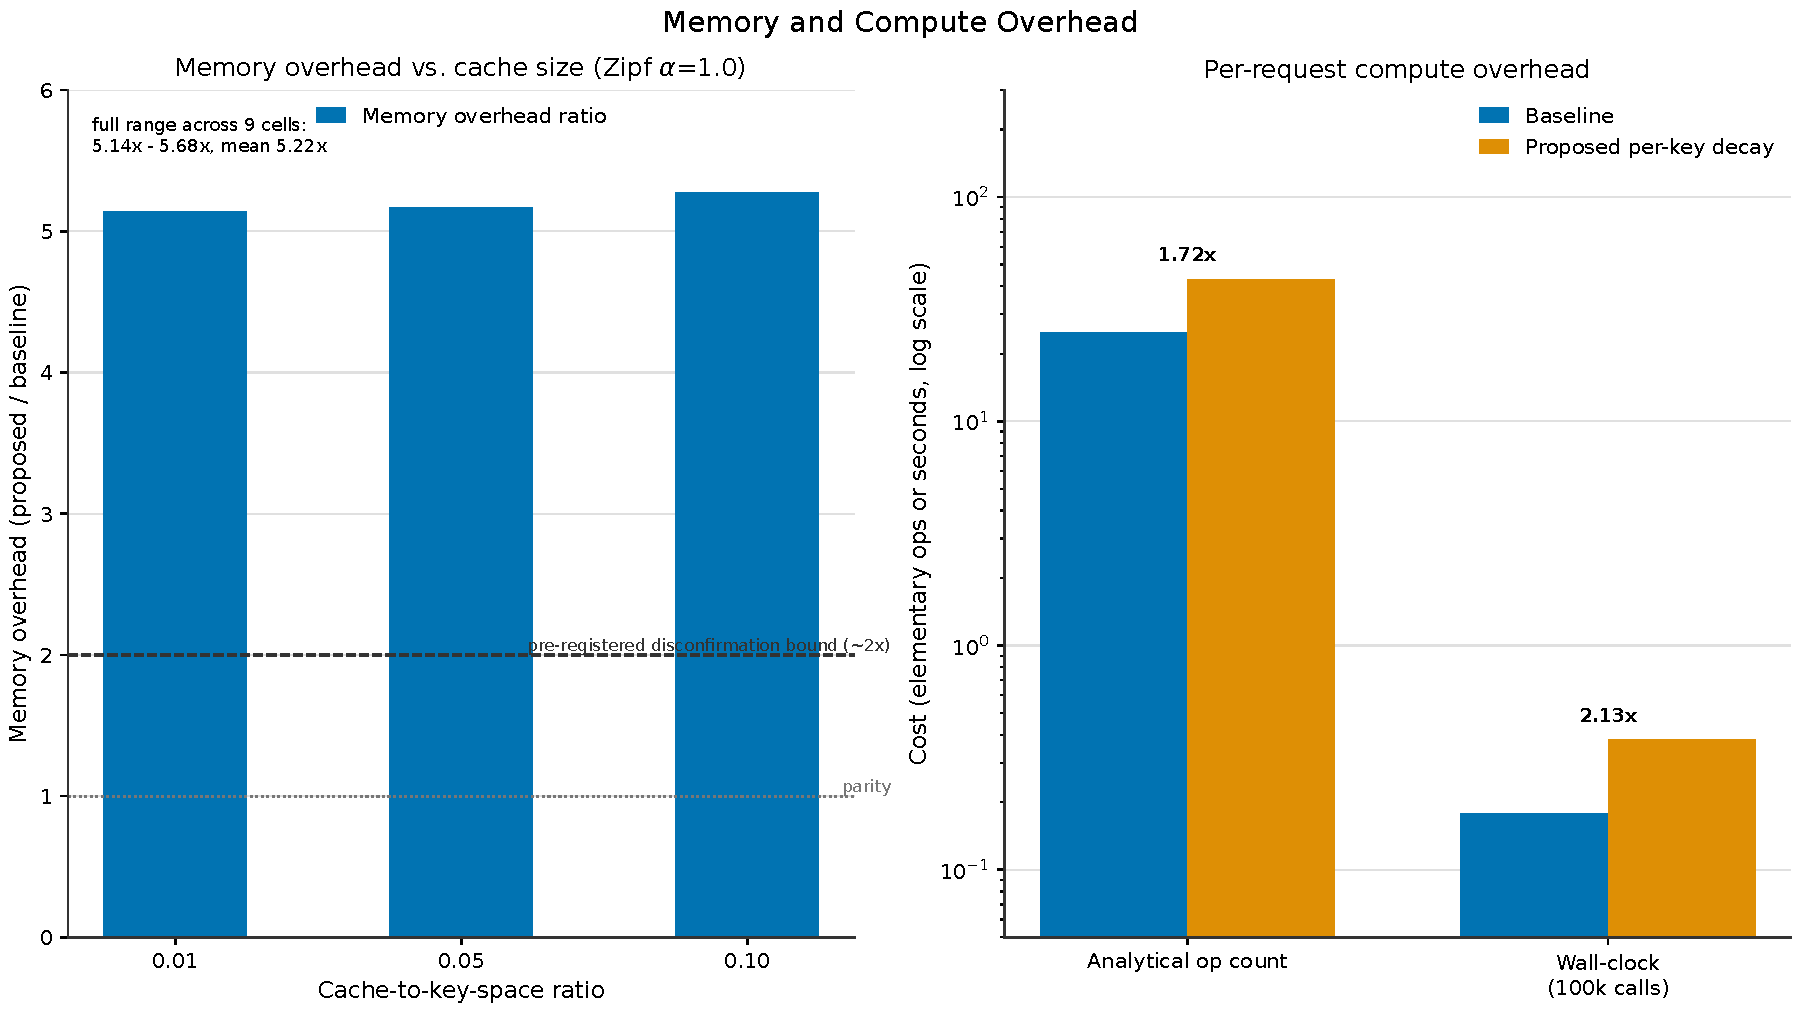
\includegraphics[width=\linewidth,height=0.85\textheight,keepaspectratio]{figures/fig_memory_v0.pdf}
  \caption{Left: memory-footprint overhead of the per-key-decay estimator relative to the global-reset baseline, at three cache-to-key-space ratios (Zipf alpha=1.0). Right: per-request compute cost, both an analytical elementary-operation count and a wall-clock microbenchmark over 100,000 calls. Both cost measures exceed the hypothesis's own pre-registered disconfirmation bound of roughly 2x memory.}
  \label{fig:memory}
\end{figure}

\textbf{Memory and compute cost.} Recomputing directly from the underlying memory-footprint measurements resolves the inconsistency the previous draft's own text and its own supporting artifact had introduced (``roughly 3-5x'' versus ``5.1-5.7x''): the corrected overhead is 5.14x at the lowest-cost cell and rises to 5.68x at the highest (mean 5.22x across all 9 (ratio, skew) cells), structurally because the proposed estimator carries three full-sized Count-Min sketches plus shadow metadata against the baseline's one sketch (Figure~\ref{fig:memory}). This exceeds the hypothesis's own pre-registered disconfirmation bound of ``no more than roughly 2x.'' An analytical operation count derived directly from the estimator code, cross-checked against a wall-clock microbenchmark (100,000 calls, 5 repeats), finds the proposed estimator issues 43 elementary per-request operations against the baseline's 25 (1.72x), and takes 2.13x as long in wall-clock time (0.380s versus 0.178s per 100,000 calls) -- the discrepancy between the two ratios reflecting Python-level object-allocation overhead in the shadow-metadata LRU rather than a difference in algorithmic work.

\section{Discussion}

Taken individually, each of the four follow-up analyses in this paper answers the specific critique it was designed to address, and none of them fully vindicates the mechanism. False-discovery correction rules out the possibility that the original 3-of-36 result was noise from testing too many conditions, which forecloses the easiest dismissal of the finding. But the short-reset ablation shows that the same win corner, examined with a cheaper alternative the original sweep never tried, gives that alternative the advantage in three of the four scenarios that made up the win corner's case -- so the corrected statistics were measuring a real effect, just largely the wrong one: mostly the effect of an under-swept baseline reset schedule, not of per-key classification. The threshold-sensitivity grid adds a second, independent reason for caution: even restricted to the one scenario (high-magnitude/high-frequency drift) where per-key decay's advantage over the baseline is real and where the short-reset ablation shows the cheaper alternative narrowing but not closing the gap, that advantage is not robust to the two CoV thresholds that route keys into tiers, holding in only 12 of 36 nearby parameter combinations.

This narrows a mechanism that was already narrow to something smaller still. The honest reading is not that per-key decay is worthless -- the high-magnitude/high-frequency drift scenario at the smallest cache-to-key-space ratio and sharpest skew is a genuine, FDR-corrected exception where the more expensive mechanism wins and a cheaper reset does not fully substitute for it -- but that this exception is a single scenario within a single corner of a 36-condition grid, sensitive to hyperparameters chosen without a dedicated tuning sweep, and unconfirmed by the one real trace available, whose lack of ground-truth drift events leaves the recovery-time question open rather than answered. An operator deciding whether to adopt per-key decay is left with a narrower recommendation than the original draft offered: consider it only for the specific combination of an extremely small cache relative to key population, high skew, and frequent, high-magnitude popularity churn, and even there, first check whether simply shortening the existing reset period gets most of the way there for free.

The cost side of the case remains unfavorable regardless of the benefit's size. A 5.14-5.68x memory multiplier and a roughly 1.7-2.1x per-request compute cost are a substantial price for an admission filter whose entire value proposition is being cheap enough to run in a shadow queue ahead of every cache decision, and neither figure moves once the benefit is shown to be narrower than originally reported. The corrected memory figure now agrees with the hypothesis's own pre-registered 5.1-5.7x estimate rather than the experiment artifact's looser ``roughly 3-5x'' restatement, and both exceed the pre-registered ``no more than roughly 2x'' disconfirmation bound outright.

\textbf{Limitations.} The short-reset ablation and the CoV threshold grid were both run only at the single win-corner cell (ratio=0.01, alpha=1.2); we have not checked whether a similarly cheap reset-schedule fix would also erode any of the other 25 statistically significant groups outside the win corner, though those groups were never claimed as practical wins in the first place (their recovery-time ratios sit above 1.0, meaning the proposed estimator is slower there, not faster). The real-trace replay establishes steady-state parity but, for lack of labeled drift events in the public Twitter release, cannot confirm or refute the recovery-time claim directly; the exploratory changepoint-based comparison is reported with that caveat rather than as independent confirmation. The compute-cost microbenchmark measures a Python reference implementation rather than a production Caffeine-style deployment in Java, so the 2.13x wall-clock ratio should be read as indicative of relative operation cost rather than as a deployment-ready latency figure. Finally, our sweep covers three discrete cache-to-key-space ratios and the ablation work above covers only the smallest; the boundary of the regime where per-key decay might still be worth its cost could sit anywhere between ratio 0.01 and 0.05, and this study does not localize it further.

\section{Conclusion}

We set out to determine whether a statistically significant, FDR-corrected recovery-time advantage for per-key CoV-based frequency decay -- found in one narrow corner of a 36-condition sweep -- reflected a genuine advantage of per-key classification, or something a cheaper baseline could match. Two targeted follow-up experiments answer that question against the mechanism: a short-reset ablation shows a single-number change to the existing global reset schedule matches or beats per-key decay in three of the four scenarios that made up the win corner's case, and a CoV threshold-sensitivity grid shows even the one scenario that survives is robust to only a third of nearby hyperparameter choices. A real-trace replay on Twitter production traffic corroborates steady-state parity but supplies no independent evidence for the recovery-time claim, for lack of labeled drift in the public release. Set against a corrected 5.14-5.68x memory overhead and a roughly 1.7-2.1x per-request compute cost, the practical conclusion is now more conservative than our own earlier draft's: per-key decay is not established as worth its overhead anywhere in the space we tested, and an operator facing this problem should first try shortening the existing reset period, which this paper shows captures most of the same benefit at a fraction of the cost. Future work should check whether the one surviving scenario holds under a properly tuned CoV threshold sweep rather than the untuned 0.5/1.5 pair used throughout, and should revisit the real-trace question once a labeled real-world drift benchmark becomes available.

\bibliographystyle{plainnat}
\bibliography{references}

\end{document}
